\documentclass{beamer}
% Nächstes Auskommentieren um jedes \pause zu 'deaktivieren'!
%\documentclass[handout]{beamer}

\usepackage{talk_BeamerColor}

\usepackage[pantoneblack7,english]{talk_wwustyle_LA}

\usepackage[ngerman]{babel}
\usepackage[utf8]{inputenc}
\usepackage[T1]{fontenc}
\usepackage{lmodern}
% --- Paket um Grafiken im Dokument einbetten zu koennen
\usepackage{graphicx}
\usepackage{caption}
\usepackage{subfigure}
\usepackage{wrapfig}
\usepackage{tikz}

% --- Pakete fuer mathematischen Textsatz
\usepackage{amsmath}
\usepackage{amssymb}
\usepackage{empheq}
\usepackage{dsfont}		
\usepackage{amstext}
\usepackage{amsfonts}
\usepackage{amsthm}
\usepackage{wasysym}

% --- Paket erweitert deutlich die Verwendung von Farben aus dem Paket 'graphicx'
\usepackage{color}

% --- Paket um Quellcode sauber zu formatieren
\usepackage{listings}

% --- Darstellung von Pseudocode und mehr (algorithmicx packages)
\usepackage{algorithm}
\usepackage{algpseudocode}

%% Physikalisches
\usepackage{nicefrac}
\usepackage{units}
\usepackage{siunitx}
\sisetup{
  inter-unit-product 	=	$\cdot$,
  fraction-function   	= 	\nicefrac,
  load-configurations 	= 	abbreviations,
  per-mode            	= 	fraction,
  separate-uncertainty	=	true,
  output-decimal-marker	=	{.}
  }   
\usepackage{isotope}

%% Aufgabenverwaltung
\usepackage[textwidth=2cm,% Breite der Todo-Eintr�ge
            textsize=footnotesize,% Schriftgr��e der Eintr�ge
            english,% deutsche Beschriftungen
            shadow,% Schlagschatten f�r Boxen (weils so h�bsch ist)
            colorinlistoftodos]{todonotes}% farbige Markierungen f�r unterschiedliche Aufgabentypen
\newcommand{\detail}[1]{\todo[color=Green,inline]{detail: #1}~}% Details k�nnten hinzugef�gt werden
\newcommand{\litcheck}[1]{\todo[color=LightSteelBlue,inline]{refcheck: #1}~}% muss noch einmal �berpr�ft werden
\newcommand{\src}[1][]{\todo[color=Tomato,inline]{reference! #1}~}% Quelle fehlt

% % Zusätzliches:
\usepackage{braket}
\usepackage{epstopdf}
\usepackage{pgfpages}
\usepackage{csquotes}

\newlength{\halftextwidth}
\setlength{\halftextwidth}{\textwidth}
\divide\halftextwidth by 2

% --- Einstellungen

\author{NiMoNa (Zwischenpräsentation) SoSe 2016}
\title{Konnektivität im Gehirn}
%\institutelogo{Logo on title frame}
%\institutelogosmall{Logo on other frames}
\subtitle{Lutz Althüser, Tobias Frohoff-Hülsmann, Victor Kärcher,\\ Lukas Splitthoff, Timo Wiedemann\\ \vspace{0.25cm} Unterstützt durch: Christian Himpe}
\date[08.06.2016]{08. Juni, 2016}

% --- Beginn des Dokuments

\begin{document}

\begin{frame}[plain]
	  \maketitle
\end{frame}

\begin{frame}{Überblick}

	  \tableofcontents
\end{frame}

\section{EEG Modell}
\begin{frame}{EEG}
\textbf{EEG = Elektroenzephalografie}
\begin{figure}
\centering
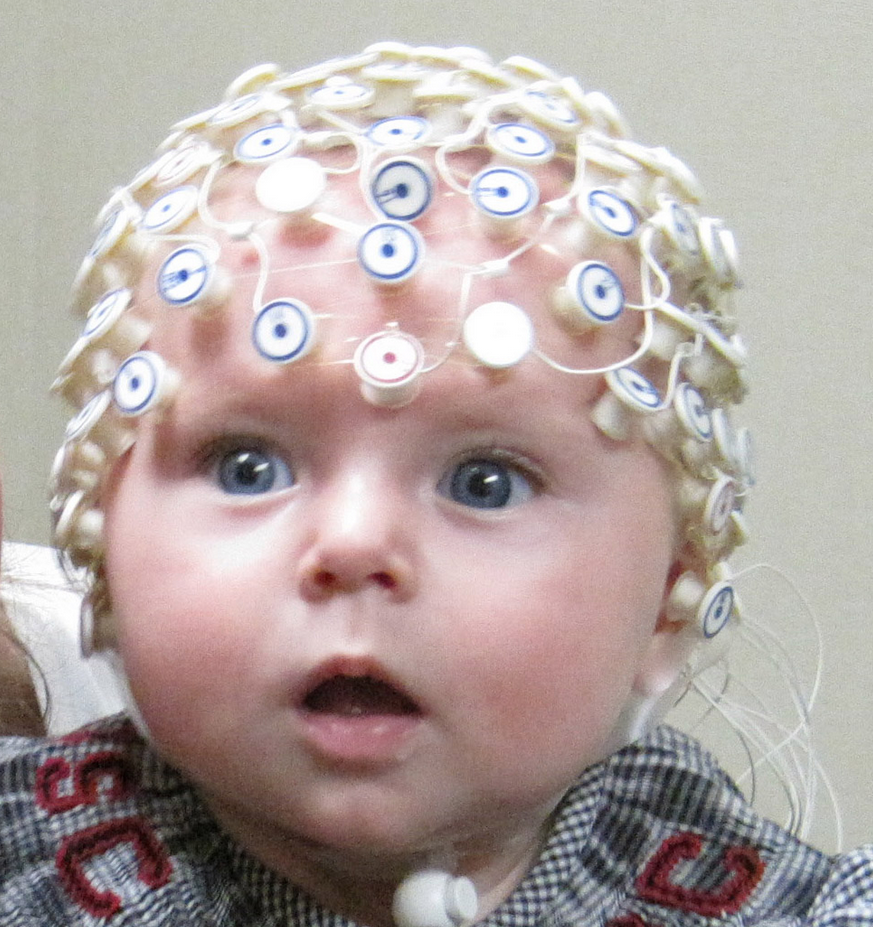
\includegraphics[scale=0.3]{res/EEGbaby.png}
\end{figure}
\end{frame}

\begin{frame}{Konzeptioneller Vergleich von fMRI- zu EEG-Modell}
\begin{tabular}{| c | c |}
\hline
\textbf{fMRI-Modell} & \textbf{EEG-Modell} \\
\hline
Verknüpfung einzelner Neuronen & Verknüpfung von Gehirnbereichen \\
&  und Subregionen untereinander \\
\hline
Taylorentwicklung & Eingangs- und \\
&  Ausgangsoperatoren \\
\hline
Gehirnaktivität = abstrakte Größe & direktes Modell für \\
biologisches Modell nötig & Potentiale und Potentialflüsse\\
\hline
\end{tabular}
\end{frame}

\begin{frame}{Das EEG-Modell}
\begin{figure}
\centering
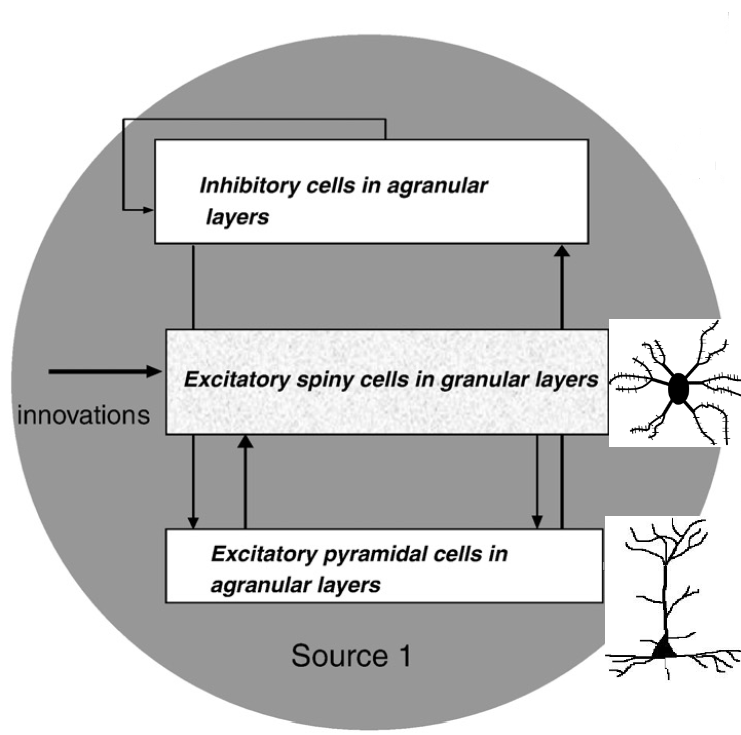
\includegraphics[scale=0.4]{res/EEGModell1.png}
\end{figure}
\end{frame}

\begin{frame}{Mathematische Realisierung - Neuroneneingang}
Physikalische Größen sind Membranpotentiale und Impulsrate\\
\begin{figure}
\centering
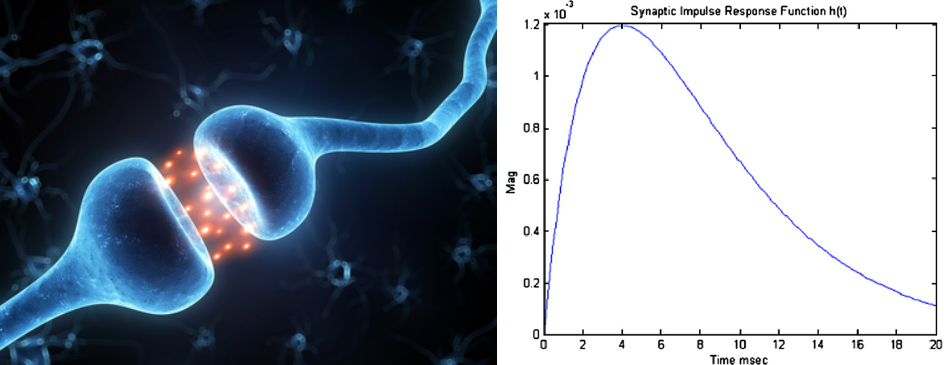
\includegraphics[scale=0.5]{res/synaptischerspalt.png}
\end{figure}
\begin{flalign*}
\text{Präsynaptische Impulsrate}&  \quad \rightarrow \quad  \text{Postsynaptisches Membranpotential}& \\
u_{ein}(t) &\quad \rightarrow \quad  v(t)=h(t)\ast u_{ein}(t) &
\end{flalign*}
\end{frame}

\begin{frame}{Mathematische Realisierung - Neuronenausgang}
\begin{figure}
\centering
\includegraphics[scale=0.21]{res/neuronausgang_sigmoid.png}
\end{figure}

\begin{flalign*}
 \text{Synaptisches Membranpotential}&  \quad \rightarrow \quad  \text{Impulsrate}& \\
v(t) &\quad \rightarrow \quad  u_{aus}(t)=S(v(t)) &
\end{flalign*}
\end{frame}

\begin{frame}{Experimente - Vergleich fMRI- mit EEG-Modell}
\begin{figure}
\centering
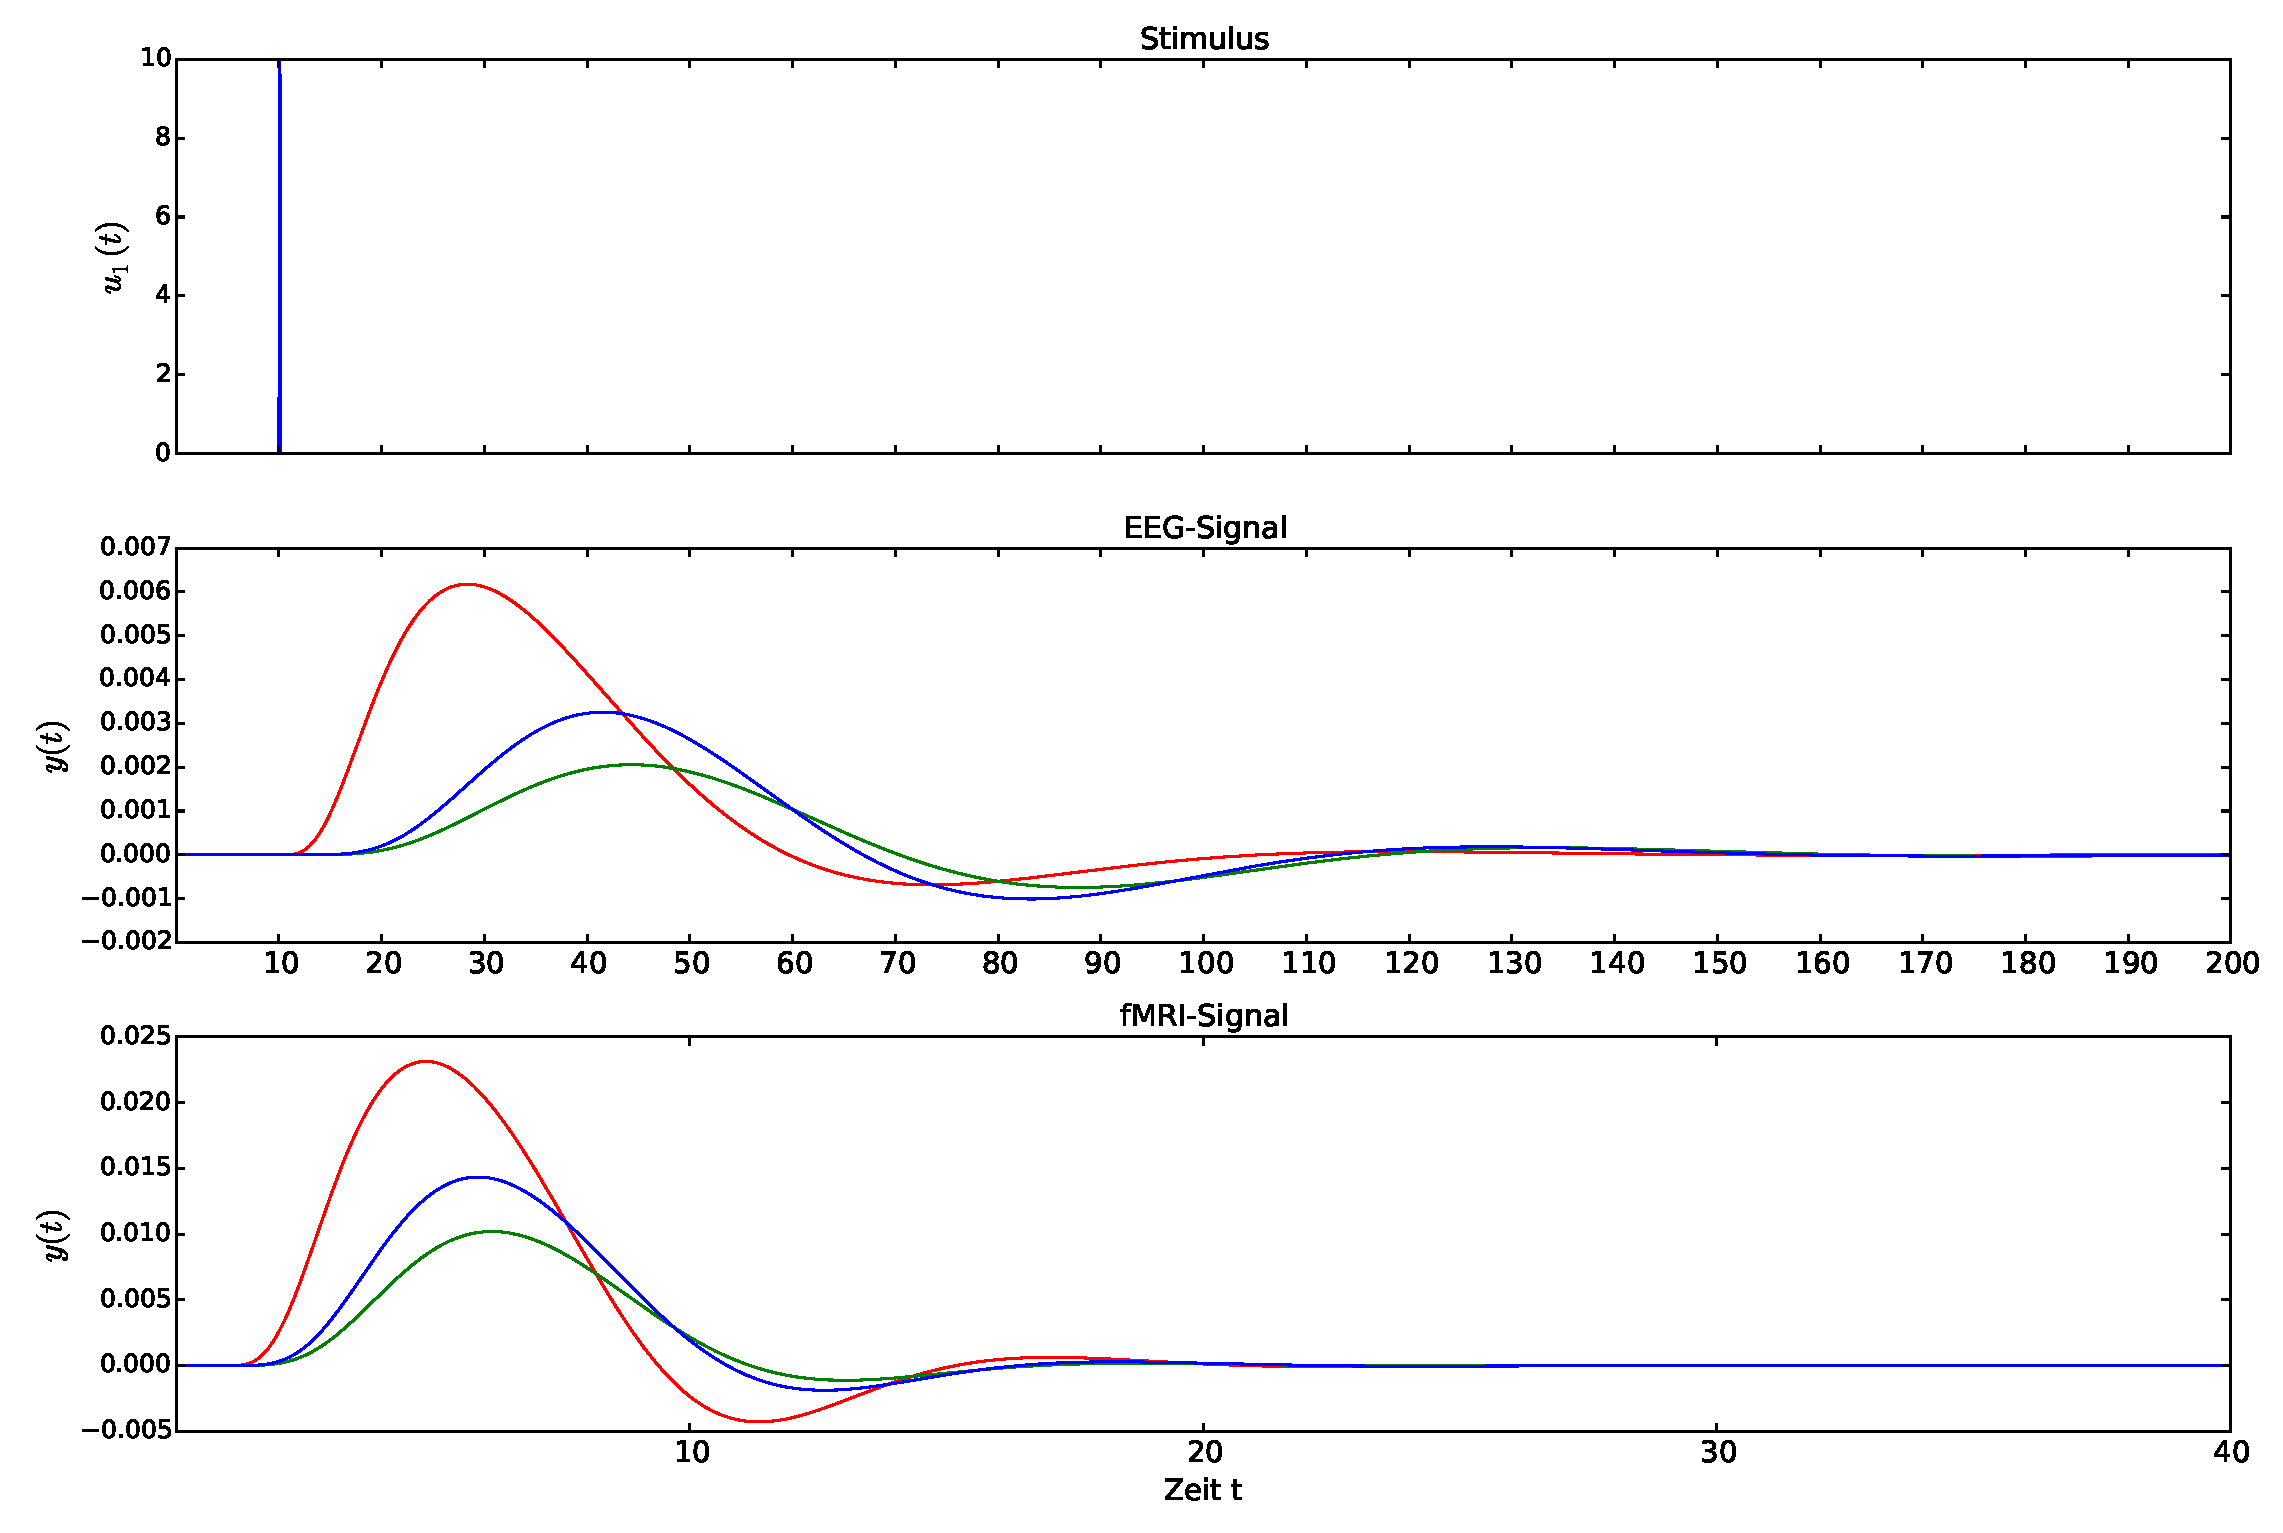
\includegraphics[scale=0.25]{res/hemo-EEG-vergleich.eps}
\end{figure}
\end{frame}

\begin{frame}{Experimente - Vergleich fMRI- mit EEG-Modell}
\begin{figure}
\centering
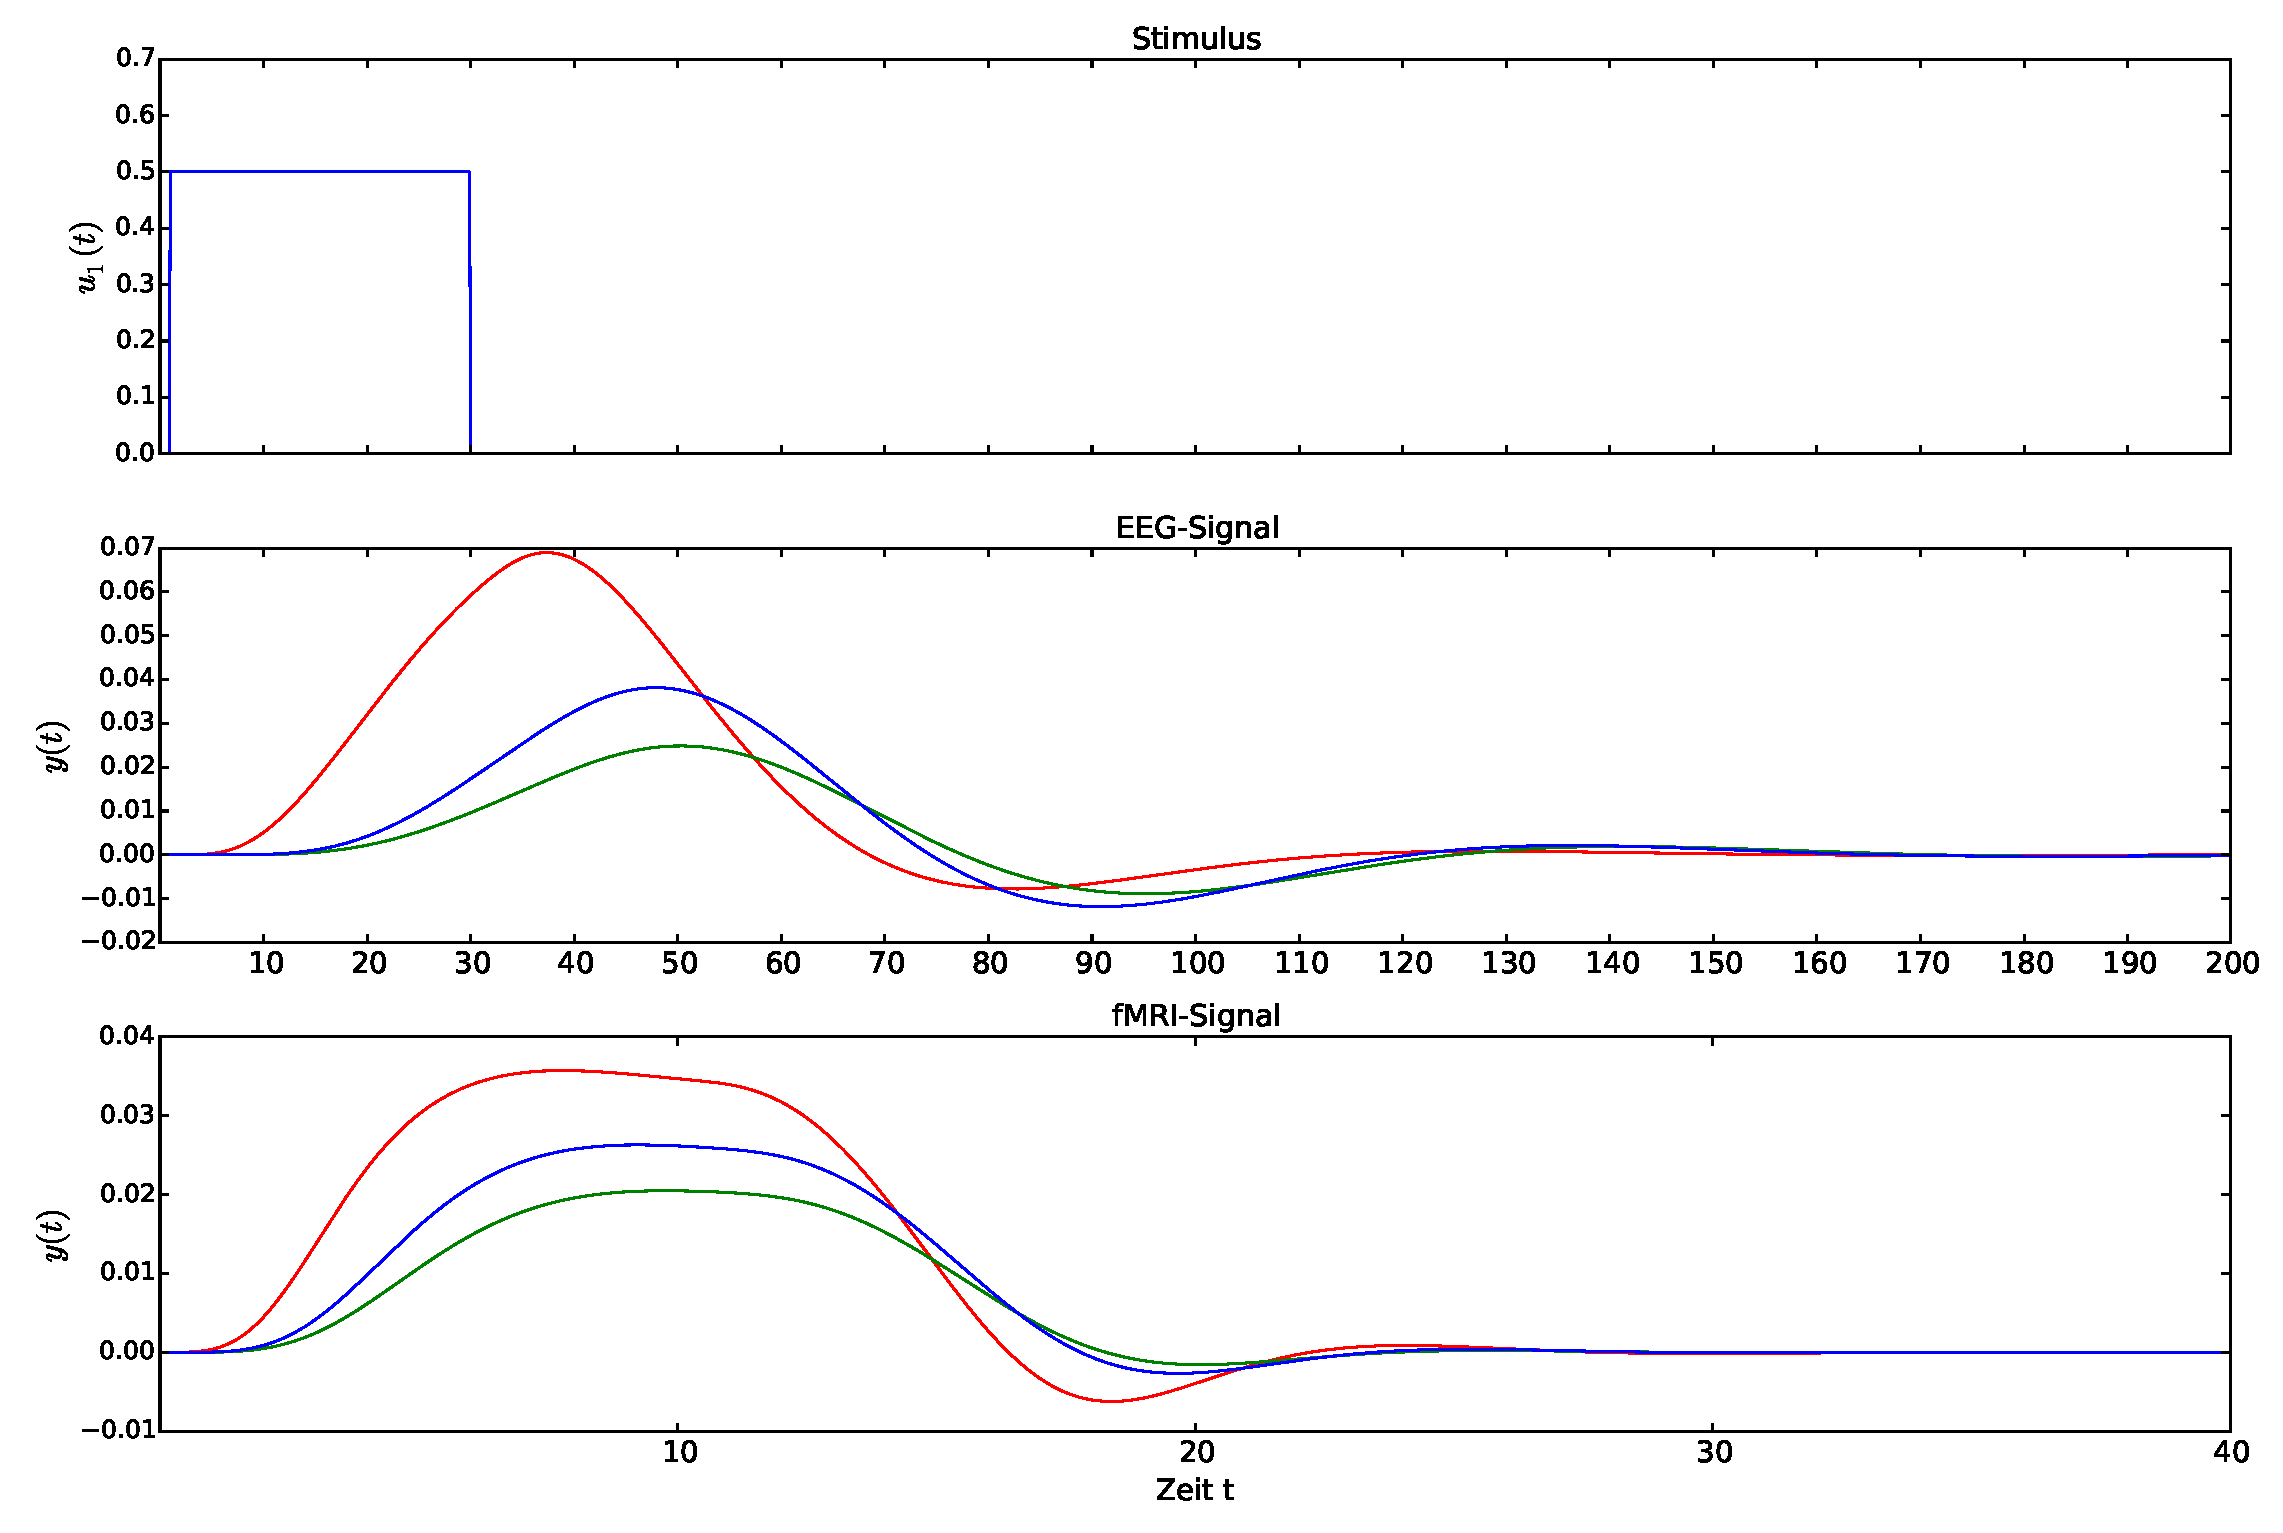
\includegraphics[scale=0.25]{res/hemo-EEG-vergleich2.eps}
\end{figure}
\end{frame}

\begin{frame}{Experimente - Vergleich fMRI- mit EEG-Modell}
\begin{figure}
\centering
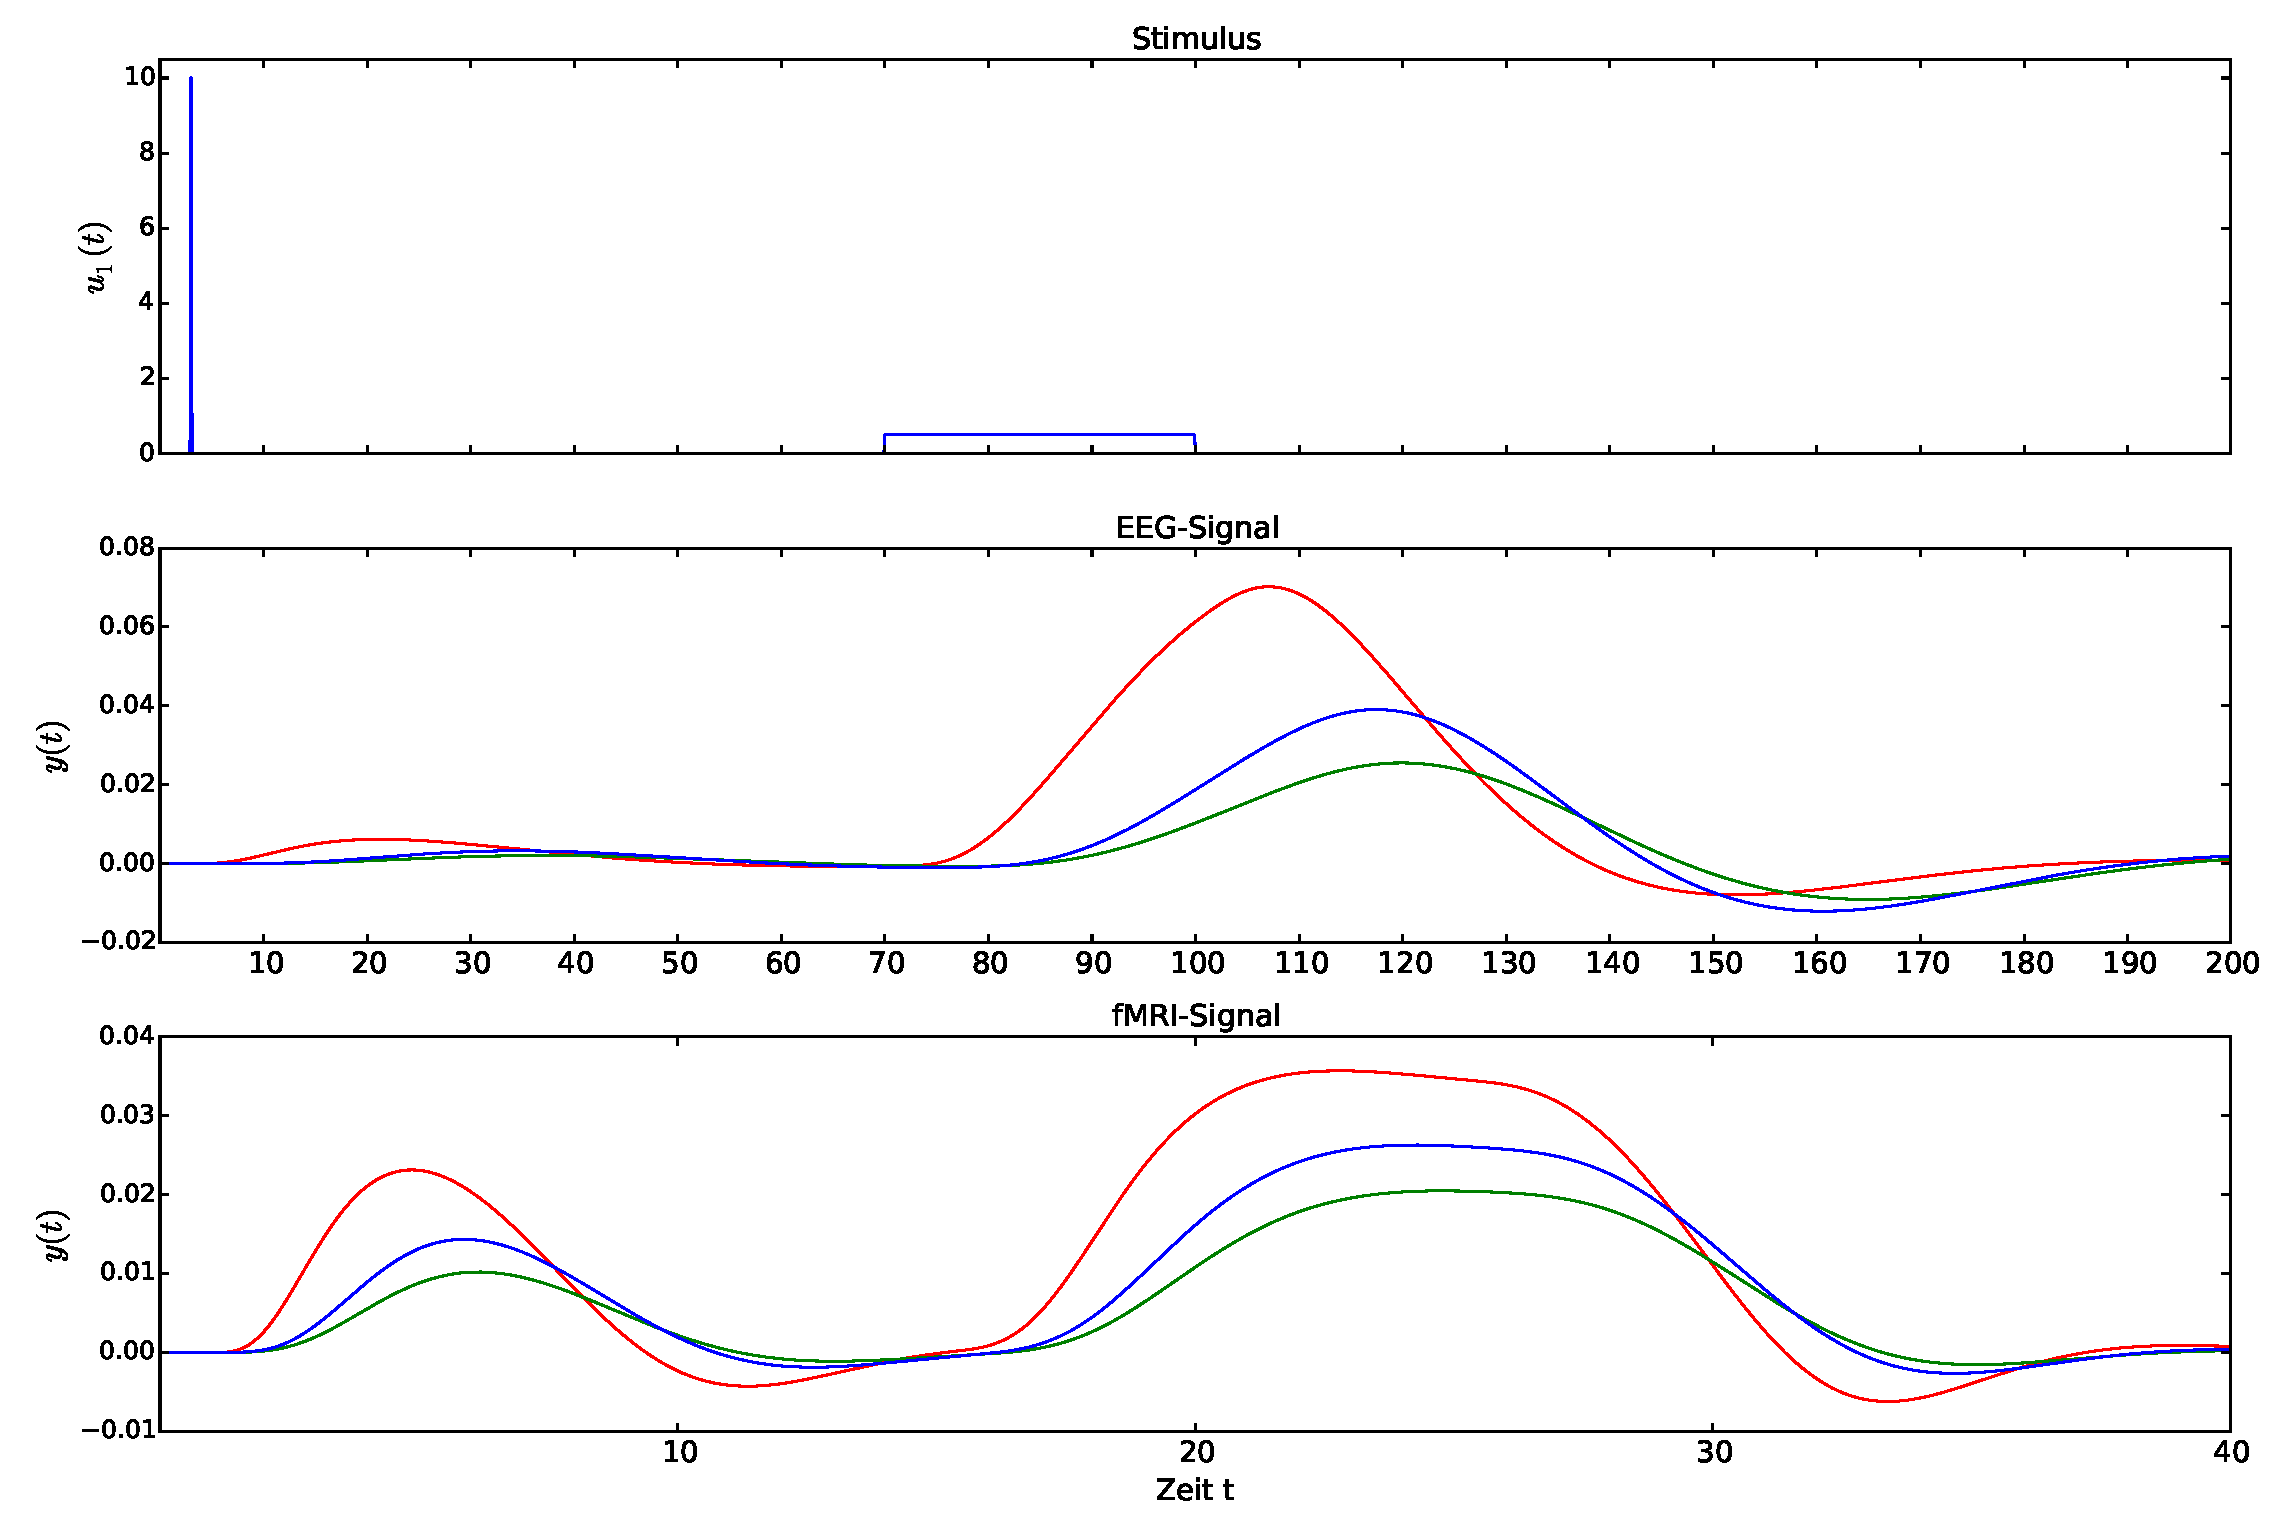
\includegraphics[scale=0.25]{res/hemo-EEG-vergleich3.eps}
\end{figure}
\end{frame}

\section{Literatur}
	\begin{frame}{Literatur}
		\begin{itemize}
			\item \textit{Dynamic causal modelling} \\ {\small K.J. Friston, L. Harrison and W. Penny / NeuroImage \textbf{4} (2003)} \\ {\footnotesize \url{web.mit.edu/swg/ImagingPubs/connectivity/Dcm_Friston.pdf}}
			\item \textit{Synaptischer Spalt}\\  {\small In: Gedankenschatz: Bewusstsein- und Persönlichkeitsentfaltung}\\{\footnotesize \url{http://gedankenschatz.de/quantenphysik-im-kopf/}}  {\tiny(Abgerufen: 6. Juli 2016, 12:28 UTC)}
						\item \textit{Sternneuronen}\\{\footnotesize \url{http://gdpsychtech.blogspot.de/2014/06/medium-spiny-neurons-msn.html}}  {\tiny(Abgerufen: 6. Juli 2016, 12:28 UTC)}	
						\item \textit{Pyramidenzellen}\\{\footnotesize \url{http://www.ruf.rice.edu/~lngbrain/Sidhya/}}  {\tiny(Abgerufen: 6. Juli 2016, 12:28 UTC)}	
						\item \textit{Aktionspotential und Neurotransmission}\\{\small In: Institut for complex Systems, Forschungszentrum Jülich}\\{\footnotesize \url{http://www.fz-juelich.de/ics/ics-4/DE/Forschungsthemen/02Biogene}}  {\tiny(Abgerufen: 6. Juli 2016, 12:28 UTC)}
												\item \textit{EEG and ERP Laboratory Experiment Demonstration}\\{\footnotesize \url{http://jerlab.psych.sc.edu/infantdevelopmentlab/pwreegdemobaby/pwrbabydemo1.htm}}  {\tiny(Abgerufen: 6. Juli 2016, 12:28 UTC)}
											%20Amine/artikel_biogene%20amine.html
			%\url{https://de.wikipedia.org/wiki/Funktionelle_Magnetresonanztomographie} 
%			\item \textit{{\small Bayesian Estimation of Dynamical Systems: An Application to fMRI}} \\ {\small K.J. Friston / NeuroImage (2002)} \\ {\footnotesize \url{www.sciencedirect.com/science/article/pii/S1053811901910444}}
		\end{itemize}
	\end{frame}

\end{document}
